%!TEX root = ../template.tex
%%%%%%%%%%%%%%%%%%%%%%%%%%%%%%%%%%%%%%%%%%%%%%%%%%%%%%%%%%%%%%%%%%%%
%% chapter3.tex
%% NOVA thesis document file
%%
%% Chapter with a short latex tutorial and examples
%%%%%%%%%%%%%%%%%%%%%%%%%%%%%%%%%%%%%%%%%%%%%%%%%%%%%%%%%%%%%%%%%%%%

\typeout{NT FILE chapter3.tex}%

\makeatletter
\newcommand{\ntifpkgloaded}{%
  \@ifpackageloaded%
}
\makeatother


\chapter{Proposal}
\label{cha:Proposal}

This Chapter aims at detailing the design and implementation of the proposed AI driven
tool, including data collection, model training, and deployment.

\section{Laboratory}
\label{sec:laboratory}

\subsection{The ABI3730xl DNA Sequencer}
The ABI3730xl DNA sequencer is a high-throughput instrument widely used in genomics for Sanger sequencing. It automates the electrophoresis and fluorescence detection steps, corresponding to steps 3 and 4 of the Sanger sequencing process (Figure \ref{fig:sanger_steps}), allowing for the simultaneous processing of 96 samples in a single run \cite{smith_capillary_sequencing,abi3730xl_overview}. By leveraging this technology, laboratories can achieve precise and efficient DNA sequencing. 
\begin{figure}[h]
\centering
\includegraphics[width=0.7\textwidth]{abi_3730xl_closed.png}
\caption{A closed ABI3730xl capillary electrophoresis DNA analyzer.}
\label{fig:abi_3730xl_closed}
\end{figure}

\begin{figure}[h]
\centering
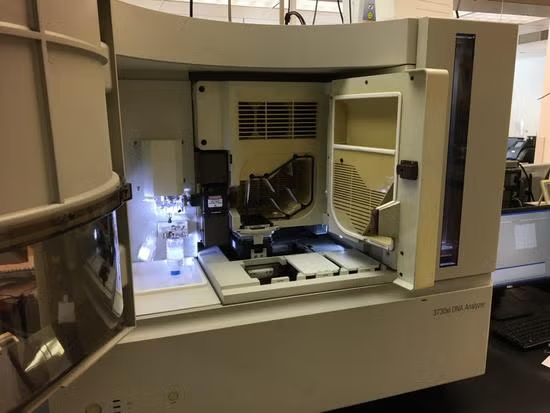
\includegraphics[width=0.7\textwidth]{abi_3730xl_opened.png}
\caption{An opened ABI3730xl capillary electrophoresis DNA analyzer.}
\label{fig:abi_3730xl_opened}
\end{figure}
\section{Data Analysis} % (fold)
\label{sec:data_analysis}

Like any Artificial Intelligence model, the efficiency that result from it's context usage stems from the data used for training. 
The data provided is customer data, that is sequenced in the ABI3730xl sequencer and afterwards outputted from it's software (elaborar mais aqui).


% section document_structure (end)


TODO